\chapter{Filtre de Bloom}
	{\huge \itshape U}n filtre de Bloom est une structure de données probabiliste compacte inventée par Burton Howard Bloom en 1970\footnote{Wikipédia}. L'avantage d'utilisation de filtre de Bloom est que cette technique nous permet de savoir avec certitude que l'élément n'est pas présenté dans l'ensemble d'élément, c'est-à-dire il ne faut pas y avoir de faux négatif mais il peut y avoir des faux positifs. On ne peut savoir qu'avec une certaine probabilité, l'élément peut être présent dans l'ensemble. Ce qui réduit d'une manière considérable les entrées lorsqu'on fait une recherche dans une masse de données. En plus, la taille de filtre est fixe et indépendante du nombre d'éléments contenus, par contre, plus déléments plus de faux positifs.
	
	En réalité, le filtre de Bloom a un structure très simple, un tableau B de \textit{m} bits associé à $i$ fonctions de hachage $h_i$, $0 \leq i \leq m - 1$ permettant de mapper tout élément de l'ensemble à une des $m$ cases du tableau. Ces fonctions de hachage ont une répartition uniforme des éléments de l'ensemble sur le tableau, et évidemment, doivent avoir une répartition différente. Au départ, le filtre représente un ensemble vide, et toutes les cases sont à 0.
	
	Pour chaque clé $k$ à ajouter à B, au lieu de se contenter de mettre à vrai la case B. $h(k)$ avec une seule fonction de hachage comme on le fait classiquement, on va mettre à vrai les $m$ cases B. $h_i(k)$. Le principe étant que la probabilité que deux clés différentes aient les mêmes $m$ valeurs pour leurs fonctions de hachage est faible.
	
	Pour savoir si une clé est présente, on s'assura que les $m$ cases de la table B correspondant aux valeurs des $m$ fonctions de hachage sont posisitionnées à $1$. Ce filtre est utile pour déterminer si un élément ne fait pas partie d'un ensemble, afin par exemple pour définir rapidement d'un traitement lourd lors de vérifier qu'une personne ne fasse pas partie d'une liste noire: d'abord, une vérification rapide avec le filtre de Bloom, puis en cas de potentiel posistif, un vérification plus certaine avec la comparaison dans la base de données.
	
	Le filtre de Bloom a quelques désavantages comme par exemple pour supprimer un élément dans l'ensemble de données, il nous faut reconstruire le filtre, en plus les faux posisitifs augmentent avec le nombre d'éléments présents dans l'ensemble. Nombreuses solutions utilisent des techniques probabilistes pour réduire le traitement d'information et leur coût.
	
	Le filtre de Bloom et leurs variantes sont largement utilisés dans divers systèmes distribués. Plusiseurs recherches récentes et beaucoup de nouveaux algorithmes ont été proposés pour les systèmes distribués qui sont directement ou indirectement basés sur Bloom filtres\cite{theory-and-practice-of-bloom-filters-for-distributed-systems}.
	
\newtheorem{algorithme}{Algorithme}
\begin{algorithme}
	Insertion dans le filtre de Bloom
\end{algorithme}

\begin{flushleft}
	\begin{framed}
		\textbf{IN:} \textit{x} objet à insérer dans le filtre de Bloom \textit{B}\\
		\textbf{FUNCTION:} \textit{insert(x)}\\
		\textbf{OUT:} $\emptyset$
		\noindent\rule{\linewidth}{0.5pt}

		\begin{tabbing}
			\textbf{for} \= $i = 0 ... k - 1$ \textbf{do}\\
					\> $j \leftarrow h_i(x)$\\
					\> \textbf{if} \= $B_j == 0$ \textbf{then}\\
					\> \> $B_j \leftarrow 1$\\
					\> \textbf{end}\\
			\textbf{end}
	    	\end{tabbing}		
	\end{framed}
\end{flushleft}
	
	Par exemple, supposons que nous souhaitions ajouter la clé "computer" dans la table B de taille 16 bits, que nous ayons 4 fonctions de hachage $ h_i, 0 \leq i < 4 $ et que $ h_0("computer") = 3$, $ h_1("computer") = 8$, $ h_2("computer") = 15$, $h_3("computer") = 10$, $h_4("computer") = 11 $. Donc, l'état de la table $ B $ après l'insertion sera:
	\begin{table}[!h]
		\centering		
		\begin{tabular}{|l|*{14}{c|}r|}
		\multicolumn{1}{c}{{\scriptsize 15}} &\multicolumn{1}{c}{}&\multicolumn{1}{c}{}&\multicolumn{1}{c}{}&\multicolumn{1}{c}{}&\multicolumn{1}{c}{}&\multicolumn{1}{c}{}&\multicolumn{1}{c}{}&\multicolumn{1}{c}{}&\multicolumn{1}{c}{}&\multicolumn{1}{c}{}&\multicolumn{1}{c}{}&\multicolumn{1}{c}{}&\multicolumn{1}{c}{}&\multicolumn{1}{c}{}&\multicolumn{1}{c}{{\scriptsize 0}}\\
		\hline
			1 & 0 & 0 & 0 & 1 & 1 & 0 & 1 & 0 & 0 & 0 & 0 & 1 & 0 & 0 & 0 \\
		\hline
		\end{tabular}
		\caption{Exemple filtre de Bloom}
		\label{filtredeBloom/exemple}
	\end{table}
	
\begin{algorithme}
	Test d'appartenance d'un élément dans le filtre
\end{algorithme}

\begin{flushleft}
	\begin{framed}
		\textbf{IN:} \emph{x} objet à tester dans le filtre de Bloom \textit{B}\\
		\textbf{FUNCTION:} \textit{ismember(x)}\\
		\textbf{OUT:} $bool$

		\noindent\rule{\linewidth}{0.5pt}

		\begin{tabbing}
			$m \leftarrow true$\\
			$i \leftarrow 0$\\
			\textbf{while} \= $m$ \&\& $i \leq k - 1$ \textbf{do}\\
					\> $j \leftarrow h_i(x)$\\
					\> \textbf{if} \= $B_j == 0$ \textbf{then}\\
					\> \> $m \leftarrow false$\\
					\> \textbf{end}\\
					\> $i \leftarrow i + 1$\\
			\textbf{end}
			\textbf{return} $m$\\
	    	\end{tabbing}		
	\end{framed}
\end{flushleft}

\begin{figure}[!htbp]
	\centering
	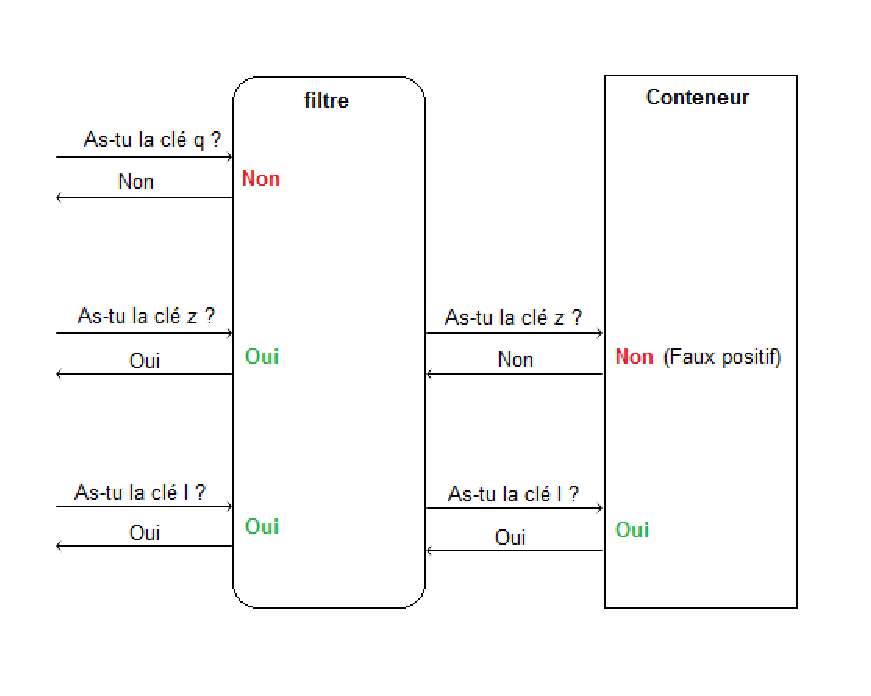
\includegraphics[width=12cm]{ismember.eps}
	\caption{isMember?}
\end{figure}	

	
	
	
	
	
	
	
	
	
	
	
	
	
	
	
	
	
	
	
	
	